\graphicspath{{figures/ISO/}}

%\setcounter{secnumdepth}{0}
\renewcommand{\theequation}{\thechapter.\arabic{equation}}
\renewcommand{\thetheorem}{\thechapter.\arabic{theorem}}
\renewcommand{\thebc}{\thechapter.\arabic{theorem}}
\renewcommand{\theeg}{\thechapter.\arabic{theorem}}
%\counterwithin{theorem}{chapter}
%\numberwithin{theorem}{chapter}


\chapter{ISO Coordinate System Notation}\label{ap:ISO}

In this text we have chosen symbols for the various polar, cylindrical and 
spherical coordinates that are standard for mathematics. There is 
another, different, set of symbols that are commonly used in the 
physical sciences and engineering. Indeed, there is an international convention, called ISO 80000-2, that specifies those symbols\footnote{It specifies more than just those symbols. See \url{https://en.wikipedia.org/wiki/ISO_31-11}
and \url{https://en.wikipedia.org/wiki/ISO/IEC_80000}. The full
ISO 80000-2 is available at \url{https://www.iso.org/standard/64973.html} --- for \$\$.}. In this appendix, we summarize the definitions and standard properties of the polar, cylindrical and spherical coordinate systems using the
ISO symbols.   

\section{Polar Coordinates}\label{ap:ISOpolar}
In the ISO convention the symbols $\rho$ and $\phi$ are used 
(instead of $r$ and $\theta$) for polar coordinates.
\begin{align*}
\rho&=\text{ the distance from }(0,0)\text{ to }(x,y)\\
\phi&=\text{ the (counter-clockwise) angle between the $x$ axis 
               and the line joining $(x,y)$ to $(0,0)$}
\end{align*}
\begin{efig}
\begin{center}
    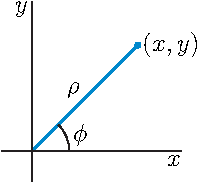
\includegraphics{polar.pdf}
\end{center}
\end{efig}
Cartesian and polar coordinates are related by
\begin{align*}
x&=\rho\cos\phi &
y&=\rho\sin\phi  \\
    \rho&=\sqrt{x^2+y^2} &
    \phi&=\arctan\frac{y}{x}
\end{align*}
The following two figures show a number of lines of constant $\phi$,
on the left, and curves of constant $\rho$, on the right.
\begin{efig}
\begin{center}
    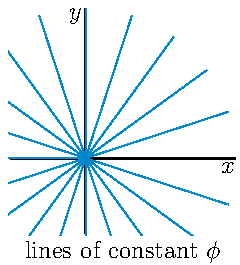
\includegraphics{polarTh.pdf}\qquad\qquad
    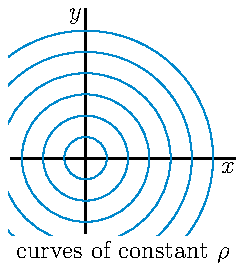
\includegraphics{polarR.pdf}
\end{center}
\end{efig}


Note that the polar angle $\phi$ is only defined up to integer multiples
of $2\pi$. For example, the point $(1,0)$ on the $x$-axis could have 
$\phi=0$, but could also have $\phi=2\pi$ or $\phi=4\pi$. It is sometimes
convenient to assign $\phi$ negative values. When $\phi<0$, the
counter-clockwise angle $\phi$ refers to the clockwise angle $|\phi|$. 
For example, the point $(0,-1)$ on the negative $y$-axis can have $\phi=-\frac{\pi}{2}$ and can also have $\phi=\frac{3\pi}{2}$.
\begin{efig}
\begin{center}
    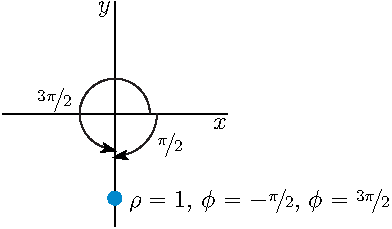
\includegraphics{polarNegTh.pdf}
\end{center}
\end{efig}



It is also sometimes convenient to extend the above definitions by saying that
$x=\rho\cos\phi$ and $y=\rho\sin\phi$ even when $\rho$ is negative. For example,
the following figure shows $(x,y)$ for $\rho=1$, $\phi=\nicefrac{\pi}{4}$
and for $\rho=-1$, $\phi=\nicefrac{\pi}{4}$.
\vadjust{
\begin{efig}
\begin{center}
    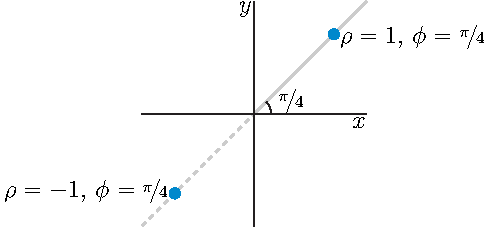
\includegraphics{polarNeg.pdf}
\end{center}
\end{efig}
}
Both points lie on the  line through the origin that makes an angle of
$45^\circ$ with the $x$-axis and both are a distance one from the origin.
But they are on opposite sides of the origin.

The area element in polar coordinates is
\begin{equation*}
\dee{A} = \rho\,\dee{\rho}\,\dee{\phi}
\end{equation*}
\begin{efig}
\begin{center}
    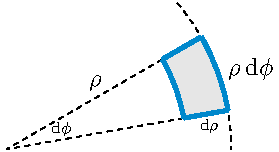
\includegraphics{polarA.pdf}
\end{center}
\end{efig}





\section{Cylindrical Coordinates}\label{ap:ISOcylCoord}
In the ISO convention the symbols $\rho$, $\phi$ and $z$ are used 
(instead of $r$, $\theta$ and $z$) for cylindrical coordinates.
\begin{align*}
\rho&=\text{ distance from }(0,0,0)\text{ to }(x,y,0)\\
\phi&=\text{ angle between the $x$ axis and the line joining $(x,y,0)$ to $(0,0,0)$}\\
z&=\text{ signed distance from }(x,y,z)
\text{ to the $xy$-plane}
\end{align*}
\begin{efig}
\begin{center}
    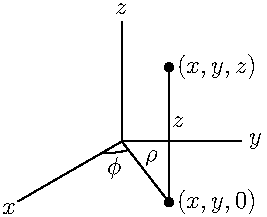
\includegraphics{cyl1.pdf}
\end{center}
\end{efig}
The cartesian and cylindrical coordinates
are related by
\begin{align*}
x&=\rho\cos\phi &
y&=\rho\sin\phi &
z&=z \\
    \rho&=\sqrt{x^2+y^2} &
    \phi&=\arctan\frac{y}{x} &
    z&=z
\end{align*}
Here are three figures showing a surface of constant $\rho$,
a surface of constant $\phi$, and a surface of constant $z$.
\begin{wfig}
\begin{center}
    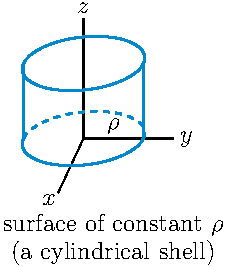
\includegraphics{cyl3.pdf}\qquad
    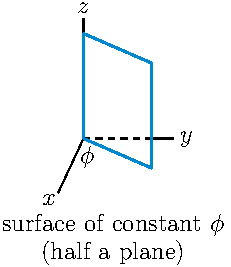
\includegraphics{cyl4.pdf}\qquad
    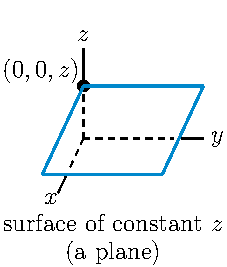
\includegraphics{cyl2.pdf}
\end{center}
\end{wfig}
Finally here is a figure showing the volume element $\dee{V}$ in
cylindrical coordinates.
\begin{efig}
\begin{center}
    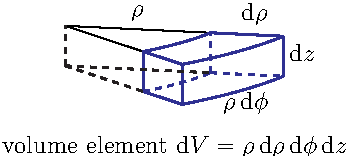
\includegraphics{cyl5.pdf}
\end{center}
\end{efig}

\section{Spherical Coordinates}\label{ap:ISOspherCoord}

In the ISO convention the symbols $r$ (instead of $\rho$), 
$\phi$ (instead of $\theta$) and $\theta$ (instead of $\phi$) are used 
for spherical coordinates.
\begin{align*}
r&=\text{ distance from }(0,0,0)\text{ to }(x,y,z)\\
\theta&=\text{ angle between the $z$ axis and the line joining $(x,y,z)$ to $(0,0,0)$} \\
\phi&=\text{ angle between the $x$ axis and the line joining $(x,y,0)$ to $(0,0,0)$}
\end{align*}
\begin{efig}
\begin{center}
    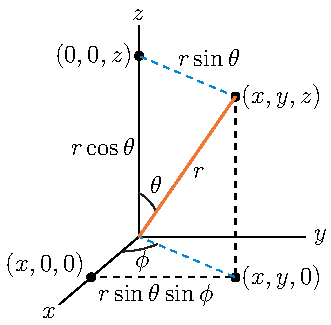
\includegraphics{spherical.pdf}
\end{center}
\end{efig}
Here are two more figures giving the side and top views of the 
previous figure.
\begin{efig}
\begin{center}
    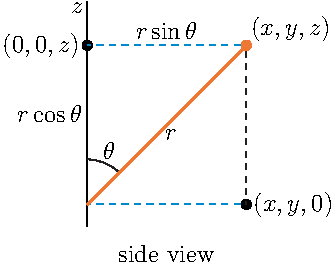
\includegraphics{sphericalSide.pdf}\qquad
    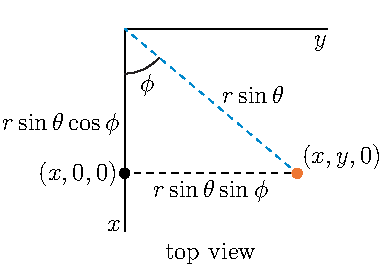
\includegraphics{sphericalTop.pdf}\qquad
\end{center}
\end{efig}
The cartesian and spherical coordinates
are related by
\begin{align*}
x&=r\sin\theta\cos\phi &
y&=r\sin\theta\sin\phi &
z&=r\cos\theta \\
 r&=\sqrt{x^2+y^2+z^2} &
 \phi&=\arctan\frac{y}{x} &
 \theta&=\arctan\frac{\sqrt{x^2+y^2}}{z}
\end{align*}
Here are three figures showing a surface of constant $r$,
a surface of constant $\phi$, and a surface of constant $\theta$.
\begin{wfig}
\begin{center}
    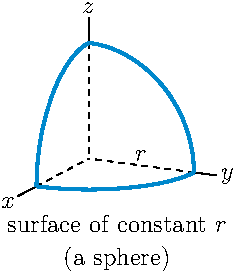
\includegraphics{spher2.pdf}\qquad
    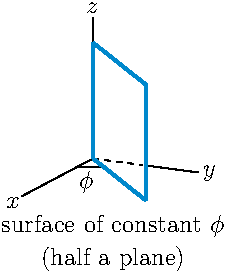
\includegraphics{spher3.pdf}\qquad
    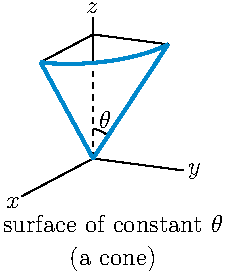
\includegraphics{spher4.pdf}
\end{center}
\end{wfig}
Finally, here is a figure showing the volume element $\dee{V}$ in
spherical coordinates
\begin{efig}
\begin{center}
    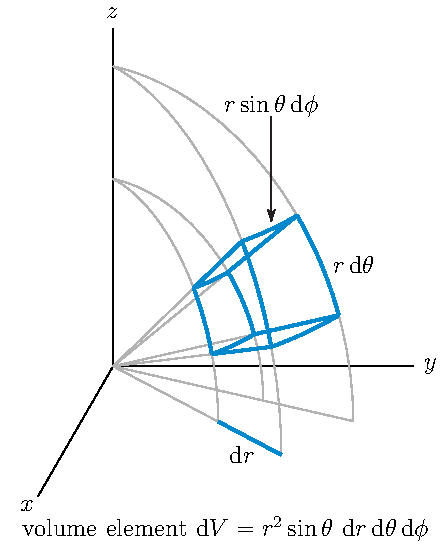
\includegraphics{spher5.pdf}
\end{center}
\end{efig}
and two extracts of the above figure to make it easier to see 
how $r\ \dee{\theta}$ and $r\sin\theta\ \dee{\phi}$ arise.
\begin{wfig}
\begin{center}
    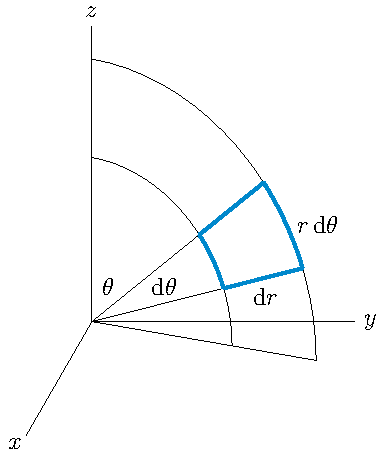
\includegraphics{spher6.pdf}\qquad
    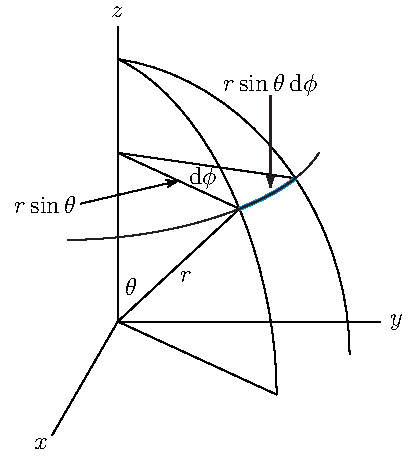
\includegraphics{spher7.pdf}
\end{center}
\end{wfig}




